\documentclass[11pt,a4paper]{article}
\ifdefined\pdfinfoomitdate\pdfinfoomitdate=1\fi
\ifdefined\pdftrailerid\pdftrailerid{}\fi
\usepackage[T1]{fontenc}
\usepackage[utf8]{inputenc}
\usepackage{lmodern,microtype}
\usepackage[margin=25mm]{geometry}
\usepackage{amsmath,amssymb,amsthm,mathtools,bm}
\usepackage{graphicx,xcolor,booktabs,array}
\usepackage{tikz}
\usetikzlibrary{arrows.meta,arrows,positioning,calc,automata}
\usepackage[numbers,sort&compress]{natbib}
\renewcommand{\bibfont}{\small}
\setlength{\bibsep}{1pt}
\usepackage{url}
\usepackage[colorlinks=true,allcolors=blue!45!black]{hyperref}
\providecommand{\openone}{\mathbf{1}}
\providecommand{\mathds}[1]{\mathbf{#1}}
\setlength{\emergencystretch}{2em}
\setlength{\parskip}{0.25em}
\allowdisplaybreaks
\newtheorem{theorem}{Theorem}
\newtheorem{lemma}[theorem]{Lemma}
\newtheorem{corollary}[theorem]{Corollary}
\newtheorem{proposition}[theorem]{Proposition}
\newtheorem{conjecture}[theorem]{Conjecture}
\definecolor{myLinkColor}{HTML}{04545c}
\definecolor{myCiteColor}{HTML}{04545c}
\definecolor{myURLColor}{HTML}{04545c}
\hypersetup{pdftitle={On the Min-Entropy Asymptotics of Binary Context Graphs},pdfauthor={Javier Blanco-Romero}}
\title{On the Min-Entropy Asymptotics of Binary Context Graphs}
\author{Javier Blanco-Romero\\\small Department of Telematic Engineering, Universidad Carlos III de Madrid,\\Legan\'es, Madrid, Spain}
\date{}
\begin{document}
\maketitle
\begin{abstract}
We study block min-entropy for binary sources with finite memory.
The context graph expresses the asymptotic rate as a minimum mean
cycle cost and supplies certificates valid at every block length.
For generalized binary autoregressive sources and mixtures of parity
rules, we give a polynomial gcd criterion for attaining the universal
noise floor.  When the rules are incompatible, polynomial relations
force defects and yield explicit weighted entropy gaps.  This argument
gives a complete solution for every source with two active lags.
We also prove exact finite-block invariance under deterministic XOR
masks, exhibit a golden-ratio spectral correction at an order-two
transition, and derive symbolic certificates for balanced negative
sources through order four.  For higher orders, we formulate a
two-run conjecture and prove that its continuum limit has a unique,
smoothly varying minimizing run ratio.
\end{abstract}

\section{Introduction}
\label{sec:introduction}

For an independent binary source, the most likely block repeats the
more likely bit.  With memory, choosing a likely bit changes the future
context and may make later outputs less likely.  Finding the most
likely block therefore requires a path through the space of histories.

An order-$p$ source has a finite context graph.  Its nodes are
length-$p$ histories, and an edge appends one bit.  Weight each edge by
the negative logarithm of its transition probability.  Products of
probabilities become sums of costs, and the most likely block becomes
the cheapest path.  Removing cycles leaves only a bounded number of
edges, so the asymptotic min-entropy rate is the minimum mean cycle
cost.  Potentials that bound every edge give finite-block guarantees
as well as certificates of cycle optimality.

Our main application is the generalized binary autoregressive process,
gbAR($p$)~\cite{jentsch2019generalized}.  At each time, the source
selects a lag and copies or flips its bit, or emits fresh noise.
With uniform noise, a transition is most likely when all selected
copy and flip instructions agree.  We first ask whether a sequence
can satisfy all these instructions at every time.  A polynomial gcd
and evaluations modulo two give a complete test, also valid for
mixtures of general parity rules.

If the rules are incompatible, a polynomial relation among them forces
at least one defect in each translated window.  Counting these windows
and weighting defects by their entropy cost gives a positive gap above
the noise floor.  For two active lags, a periodic word attains this
bound, solving the problem for every choice of lags, signs, and weights.
For more rules, the distribution of simultaneous defects matters.
We obtain further exact families and isolate a two-run candidate for
the balanced purely negative model at general order.

\subsection*{Related work}

Min-entropy and average conditional min-entropy are standard measures
of guessing probability~\cite{renyi1961measures,dodis2004fuzzy}, and
predictors provide operational upper bounds on source
min-entropy~\cite{kelsey2015predictive}.  The gbAR model belongs to the
mixture-based discrete autoregressive family introduced by Jacobs and
Lewis and extended to signed coefficients by Jentsch and
Reichmann~\cite{jacobs1978discrete,jentsch2019generalized}.  Our
previous work studied finite-block and predictor-based min-entropy for
gbAR sources~\cite{blanco2025machine}; the present paper isolates the
exact asymptotic structure.

The finite-state part uses classical graph and spectral tools.  Minimum
mean cycles, circulation duality, and max-plus cyclicity give the rate,
the reduced-cost certificate, and the eventual finite-block
correction~\cite{karp1978characterization,baccelli1992synchronization}.
The R\'enyi rate is a Perron-root formula~\cite{rached2001renyi}.  In
ergodic-optimization language, minimum cycles support minimizing
measures and reduced-cost potentials are finite-state sub-actions
~\cite{jenkinson2006ergodic,jenkinson2019ergodic,bousch2000lepoisson,
garibaldi2017ergodic}.  The large-order limit is the zero-temperature
limit of a locally
constant potential, whose spectral asymptotics and Gibbs selection
are well studied~\cite{bremont2003gibbs,chazottes2011zero}.

The homogeneous parity systems define one-dimensional group shifts;
compatible affine systems are their translates.  Both can be read as convolutional
constraints~\cite{schmidt1995dynamical,forney1970convolutional}.  Gauge
removal and frustrated sign patterns parallel the Mattis and Toulouse
pictures in spin systems~\cite{mattis1976solvable,toulouse1977frustration}.
The uniform-noise bounds place gbAR sources within the usual
Santha--Vazirani interval description of weak randomness
~\cite{santha1986generating,chor1988unbiased}.  At weak coupling, the
balanced negative family becomes a Max-Cut problem on circulant graphs
~\cite{poljak1992max}.

Our main results are the algebraic noise-floor criterion, weighted
entropy bounds from incompatible rules, and the complete two-lag
formula.  Exact gauge invariance and symbolic certificates simplify
further families.  The finite-state spectral and periodicity results
provide the foundation and an explicit application at the order-two
transition.  The higher-order analysis gives finite-order formulas
and a unique continuum optimum for the two-run candidate.

Section~\ref{sec:finite_state} develops the finite-state theory.
Section~\ref{sec:signed_rules} gives the signed-lag and parity-rule
formulation.  Section~\ref{sec:families} collects the gbAR formulas and
the higher-order conjecture.

\section{Finite-State Min-Entropy}
\label{sec:finite_state}

Throughout, $\log$ means $\log_2$, $\ln$ is the natural logarithm,
and $\oplus$ denotes addition modulo two (XOR).  Fix a stationary
binary source $X=(X_t)_{t\in\mathbb Z}$ whose conditional law depends
on at most $p$ preceding bits, where $p\ge1$ is an integer.  Its context space is
$\mathcal C_p=\{0,1\}^p$, with oldest-first context
\[
    U_t=(X_{t-p},\ldots,X_{t-1}).
\]
Thus lag $i$ is component $u_{p+1-i}$ of a context $u$.  Write
$P(x\mid u)=P(X_t=x\mid U_t=u)$ for the transition probability.
Appending $x\in\{0,1\}$ updates the context by
\[
    T(u,x)=(u_2,\ldots,u_p,x).
\]
Let $\pi$ be the stationary context law and
$\mathcal S_p=\{u\in\mathcal C_p:\pi(u)>0\}$ its support.
All context maxima and sums below are over $\mathcal S_p$.

\subsection{Block guessing and the context graph}

The one-step guessability at $u$ is $g_1(u)=\max_xP(x\mid u)$.
For a finite-valued random variable $Z$, its min-entropy is
\[
    H_\infty(Z)=-\log\max_zP(Z=z).
\]
For $n\ge1$, write $X_t^{t+n-1}=(X_t,\ldots,X_{t+n-1})$ for an
output block and $x_1^n\in\{0,1\}^n$ for a realization.
The worst-context and average-conditional min-entropies per symbol are
\begin{align}
    h_\infty^{\mathrm{worst}}(n)
    &:=-\frac1n\log\max_{\substack{u\in\mathcal S_p\\x_1^n\in\{0,1\}^n}}
       P(X_t^{t+n-1}=x_1^n\mid U_t=u),
    \label{eq:worst_rate}\\
    \widetilde h_\infty^{\mathrm{avg}}(n)
    &:=-\frac1n\log\sum_{u\in\mathcal S_p}\pi(u)
       \max_{x_1^n}P(X_t^{t+n-1}=x_1^n\mid U_t=u).
    \label{eq:avg_rate}
\end{align}
They satisfy
\begin{equation}
\label{eq:block_sandwich}
    h_\infty^{\mathrm{worst}}(n)
    \le \widetilde h_\infty^{\mathrm{avg}}(n)
    \le \frac1nH_\infty(X_t^{t+n-1})
    \le h_\infty^{\mathrm{worst}}(n)+\frac{\Delta_0}{n},
\end{equation}
where $\Delta_0=-\log\min_{u\in\mathcal S_p}\pi(u)$.  The first two
inequalities follow by averaging conditional guessing probabilities.
For the last, the unconditional probability of a best conditional
block is at least its conditional probability times the stationary
weight of its starting context.  Hence the three limits agree whenever
one exists; we denote this common rate by $h_\infty$.
We use $H_*(n)$ for any of the three unnormalized quantities
$n h_\infty^{\mathrm{worst}}(n)$,
$n\widetilde h_\infty^{\mathrm{avg}}(n)$, and $H_\infty(X_1^n)$
when the same assertion applies to all three.

\paragraph{The flat SIMTP benchmark.}
An order-$p$ chain is state-independent maximum transition probability
(SIMTP) when $g_1(u)=P_{\max}$ for every $u\in\mathcal S_p$.  In that
case, from each context there is an outgoing edge of probability
$P_{\max}$, so a most likely continuation can keep paying the same cost
at every step.  Conversely, no continuation can have larger
probability.  Hence, for every $n$,
\begin{equation}
\label{eq:simtp_benchmark}
    h_\infty^{\mathrm{worst}}(n)
    =\widetilde h_\infty^{\mathrm{avg}}(n)
    =-\log P_{\max},
    \qquad
    h_\infty=-\log P_{\max}.
\end{equation}
The unconditional stationary block entropy can still carry a bounded
initial-state correction.  SIMTP is therefore the flat case in which
context compatibility adds no asymptotic cost.  When $g_1$ varies,
locally maximizing edges still contain a cycle, but its mean cost
need not be optimal.  SIMTP can also be detected at one step.  The equality
$h_\infty^{\mathrm{worst}}(1)=\widetilde
h_\infty^{\mathrm{avg}}(1)$ holds only when the maximum of $g_1(u)$
equals its stationary average, which forces $g_1$ to be constant.

The context graph has node set $\mathcal S_p$ and one edge
$u\xrightarrow{x}T(u,x)$ for every positive transition probability.
We attach the edge cost
\begin{equation}
\label{eq:edge_cost}
    c(u,x)=-\log P(X_t=x\mid U_t=u).
\end{equation}
A directed cycle
$C=(u_0\xrightarrow{x_0}u_1,\ldots,
 u_{\ell-1}\xrightarrow{x_{\ell-1}}u_0)$
has mean cost
\[
    \mu(C)=\frac1\ell\sum_{j=0}^{\ell-1}c(u_j,x_j).
\]
The minimum local cost $\min_u[-\log g_1(u)]$ is a lower bound on
every mean cycle cost.  Attaining it requires a cycle made entirely of
edges with that global minimum cost.

\begin{theorem}[Cycle formula and dual certificate]
\label{thm:cycle_and_dual}
Assume the context graph is strongly connected, so every context can
reach every other context, and set
\[
    \mu^*=\min_C\mu(C),
\]
where the minimum is over directed cycles.  Then
\[
    h_\infty=\mu^*.
\]
A minimizing simple cycle has length at most $|\mathcal S_p|\le2^p$.
Moreover, if a function $\varphi:\mathcal S_p\to\mathbb R$ and a
real number $\lambda$ satisfy
\begin{equation}
\label{eq:dual_certificate}
    c(u,x)+\varphi(u)-\varphi(T(u,x))\ge\lambda
\end{equation}
for every edge, then $h_\infty\ge\lambda$.  Equality holds if the tight
edges, meaning those for which \eqref{eq:dual_certificate} holds with
equality, contain a directed cycle.  Conversely, a potential satisfying
\eqref{eq:dual_certificate} exists for $\lambda=\mu^*$.
\end{theorem}

\begin{proof}
For a fixed starting context, a continuation has probability equal to
the product of its edge probabilities.  Its negative logarithm is
therefore the path cost.  Strong connectivity lets a path reach a
minimum mean cycle and repeat it, with bounded initial and final
costs.  This gives an asymptotic cost at most $\mu^*$.

For the reverse bound, remove closed portions of any length-$n$ path
until the remaining path is simple.  Each removed portion decomposes
into cycles, all of mean at least $\mu^*$.  At most
$|\mathcal S_p|-1$ edges remain, and their costs are nonnegative, so
\[
    \text{path cost}\ge\mu^*(n-|\mathcal S_p|+1).
\]
Division by $n$ proves convergence, and \eqref{eq:block_sandwich}
transfers it to all three entropy notions.  Decomposing a closed walk
also shows that some simple cycle has no larger mean; its length is
at most $|\mathcal S_p|$.

Summing \eqref{eq:dual_certificate} around a cycle cancels the
potential differences and bounds its mean cost below by $\lambda$.
A cycle of tight edges attains equality.  To construct an optimal
potential, subtract $\mu^*$ from every edge cost.  All cycles now
have nonnegative cost.  Add an auxiliary node with a zero-cost edge
to every context, and let $\varphi(v)$ be the shortest-path distance
from that node to $v$.  These distances are finite because there is
no negative cycle.  Extending a shortest path by one edge gives
\[
    \varphi(v)\le\varphi(u)+c(u,x)-\mu^*,
\]
which is the required inequality.
\end{proof}

A potential redistributes edge costs while preserving every cycle
cost.  This is the dual certificate for the minimum mean cycle problem.
Karp's algorithm computes the rate in $O(NM)$ operations for $N$
nodes and $M$ edges~\cite{karp1978characterization}.  A full binary
context graph has $N=2^p$ and $M=2^{p+1}$, giving $O(4^p)$ complexity.

\begin{corollary}[Finite-block certificate]
\label{cor:finite_block_certificate}
If $\varphi$ satisfies \eqref{eq:dual_certificate}, then, for every
$n\ge1$,
\begin{equation}
\label{eq:finite_block_certificate}
    H_*(n)\ge n\lambda-\operatorname{osc}(\varphi),
    \qquad
    \operatorname{osc}(\varphi)=\max_u\varphi(u)-\min_u\varphi(u).
\end{equation}
\end{corollary}

\begin{proof}
Along a path $u_0\to\cdots\to u_n$, telescoping gives
$\sum c\ge n\lambda+\varphi(u_n)-\varphi(u_0)$.
Minimize over paths and use \eqref{eq:block_sandwich}.
\end{proof}

The certificate applies before any asymptotic regime.  If every edge
inequality is rigorously bounded below by $\lambda-\varepsilon$,
with $\varepsilon\ge0$, replace $\lambda$ by
$\lambda-\varepsilon$ in \eqref{eq:finite_block_certificate}.

\paragraph{A four-state example.}
Consider a source that flips lag $1$ or lag $2$, each with
probability $0.3$, and otherwise emits a fair bit with probability
$0.4$.  This is the purely negative gbAR(2) model with coefficients
$\alpha_1=\alpha_2=-0.3$ and noise weight $\beta=0.4$.  Its
transition table is
\begin{center}
\scriptsize
\begin{tabular}{cccccc}
\toprule
Context $u$ & $P(0\mid u)$ & $P(1\mid u)$ & $g_1(u)$ & $-\log g_1(u)$ & Best $x$\\
\midrule
$00$ & $0.20$ & $0.80$ & $0.80$ & $0.322$ & $1$\\
$01$ & $0.50$ & $0.50$ & $0.50$ & $1.000$ & either\\
$10$ & $0.50$ & $0.50$ & $0.50$ & $1.000$ & either\\
$11$ & $0.80$ & $0.20$ & $0.80$ & $0.322$ & $0$\\
\bottomrule
\end{tabular}
\end{center}
Figure~\ref{fig:gbar2_context_graph} shows the full context graph.  The
solid period-four cycle
$00\to01\to11\to10\to00$ has mean cost
$(0.322+1+0.322+1)/4=0.661$ and is the minimum-mean cycle.  An edge of probability $0.8$ always
leaves a unanimous context
for a mixed one, where the next edge has probability $0.5$.  This is the
simplest example in which the minimum local prediction cost does not
determine the asymptotic rate.

\begin{figure}[tbp]
\centering
\begin{tikzpicture}[
    >=stealth',
    auto,
    node distance=2.7cm,
    thick,
    hnode/.style={circle,draw,fill=red!12,minimum size=1.05cm},
    lnode/.style={circle,draw,fill=blue!12,minimum size=1.05cm},
    optimal/.style={->,very thick,draw=myLinkColor},
    other/.style={->,thin,dashed,draw=black!55}
]
    \node[hnode] (00) {$00$};
    \node[lnode] (01) [right of=00] {$01$};
    \node[lnode] (10) [below of=00] {$10$};
    \node[hnode] (11) [right of=10] {$11$};

    \draw[optimal] (00) edge[bend left=15] node[above]{$x=1$} (01);
    \draw[optimal] (01) edge[bend left=15] node[right]{$x=1$} (11);
    \draw[optimal] (11) edge[bend left=15] node[below]{$x=0$} (10);
    \draw[optimal] (10) edge[bend left=15] node[left]{$x=0$} (00);

    \draw[other] (00) edge[loop left] node{$x=0$} (00);
    \draw[other] (11) edge[loop right] node{$x=1$} (11);
    \draw[other] (01) edge node[above left]{$x=0$} (10);
    \draw[other] (10) edge node[below right]{$x=1$} (01);
\end{tikzpicture}
\caption{Context graph of the balanced negative gbAR(2) example.  Red
nodes have local cost $0.322$ and blue nodes have local cost $1$.  The
solid edges form the minimum-mean cycle; dashed edges are the remaining
transitions.}
\label{fig:gbar2_context_graph}
\end{figure}

\subsection{R\'enyi rates and finite-block corrections}
\label{subsec:renyi_finite}

Assume throughout this subsection that the context chain on
$\mathcal S_p$ is irreducible, meaning its graph is strongly connected.  For $q>0$, $q\ne1$, define
\[
    H_q(Z)=\frac{1}{1-q}\log\sum_zP(Z=z)^q,
    \qquad h_q=\lim_{n\to\infty}\frac{H_q(X_1^n)}n.
\]
The limits at $q=1$ and $q\to\infty$ give Shannon entropy and
min-entropy.  The standard spectral formula is
\begin{equation}
\label{eq:renyi_spectral}
    h_q=\frac{1}{1-q}\log\lambda_q,
\end{equation}
where $\lambda_q$ is the Perron root (the spectral radius) of
\[
    (M_q)_{u,T(u,x)}=P(x\mid u)^q=2^{-q c(u,x)}
\]
on allowed edges, with all other entries zero
~\cite{rached2001renyi}.  Fixing the first $p$ output bits fixes the
context, so boundary probabilities do not change this entropy rate.

Fix an optimal potential $\varphi$ in
\eqref{eq:dual_certificate} with $\lambda=\mu^*$ and define the reduced
cost of an edge $e:u\to v$, writing $c(e)=c(u,x)$,
\[
    r(e)=c(e)+\varphi(u)-\varphi(v)-\mu^*\ge0.
\]
Call an edge \emph{tight} when $r(e)=0$, and let $K$ be the adjacency
matrix of the tight-edge subgraph.  Its $(u,v)$ entry is one when a tight
edge goes from $u$ to $v$, and zero otherwise.  The critical graph
consists of the nodes and edges that lie on at least one minimum mean
cycle.  Equivalently, it is the part of the tight-edge subgraph that
belongs to directed cycles; tight edges outside it cannot contribute
to a closed walk.  We write $\rho(K)$ for the spectral radius of $K$.
Deleting tight edges that lie on no cycle does not change this spectral
radius.

\begin{proposition}[Large-order R\'enyi rate]
\label{prop:large_order_renyi}
For every $q>1$,
\begin{equation}
\label{eq:renyi_bound}
    0\le h_q-h_\infty\le\frac{h_\infty}{q-1}\le\frac{1}{q-1}.
\end{equation}
More precisely,
\begin{equation}
\label{eq:renyi_correction}
    \lambda_q=2^{-q h_\infty}\bigl(\rho(K)+o(1)\bigr),
    \qquad
    h_q=h_\infty+
    \frac{h_\infty-\log\rho(K)}{q-1}
    +o(q^{-1}).
\end{equation}
\end{proposition}

\begin{proof}
Let $C$ be a minimum-mean cycle of length $\ell$, based at $u$.
The diagonal entry $(M_q^\ell)_{u,u}$ sums the weights of all closed
paths of length $\ell$ from $u$.  The single contribution from $C$ is
\[
    \prod_{e\in C}2^{-q c(e)}=2^{-q\ell h_\infty}.
\]
Since $\rho(M_q^\ell)=\lambda_q^\ell$ is at least this diagonal
entry, $\lambda_q\ge2^{-q h_\infty}$.

Since $1-q<0$, this lower bound on $\lambda_q$ gives
$h_q\le qh_\infty/(q-1)$.  Monotonicity of R\'enyi entropy gives
$h_q\ge h_\infty$.  Finally, $h_\infty\le1$ because a binary block
of length $n$ has at most $2^n$ possible values.  This proves
\eqref{eq:renyi_bound}.

For the correction, let
$D_q=\operatorname{diag}(2^{-q\varphi(u)})$.  Conjugation preserves
eigenvalues, and the normalized matrix has entries
\[
    \bigl(2^{q h_\infty}D_qM_qD_q^{-1}\bigr)_{u,v}
    =2^{-q r(e)}.
\]
They tend to one on tight edges and zero elsewhere.  The matrix
therefore converges to $K$.  Continuity of the spectral radius in
finite dimension gives
$2^{q h_\infty}\lambda_q\to\rho(K)$, which is positive because
$K$ contains a minimum mean cycle.  Taking logarithms proves
\eqref{eq:renyi_correction}.
\end{proof}

We now turn to exact finite-block behavior.  Two nodes are in the same
strongly connected component when each can be reached from the other
by a directed path.  For each strongly connected component of the
critical graph, take the greatest common divisor of the lengths of all
its directed cycles.  Let $\gamma$ be the least common multiple of
these componentwise gcds.  This integer is the cyclicity of the
critical graph.

For $u\in\mathcal S_p$ and $n\ge0$, let $D_u(n)$ be the cheapest
length-$n$ continuation cost from $u$, with $D_u(0)=0$.

\begin{proposition}[Eventual periodicity of block costs]
\label{prop:block_periodicity}
There is $N_0$ such that
\begin{equation}
\label{eq:continuation_periodicity}
    D_u(n+\gamma)=D_u(n)+\gamma h_\infty
\end{equation}
for every $u$ and every $n\ge N_0$.  Consequently, after subtracting
$n h_\infty$, the worst-context, average-conditional, and stationary
unconditional block min-entropies are eventually periodic, with period
dividing $\gamma$.
\end{proposition}

\begin{proof}
Define the min-plus context matrix $A$ by
\[
    A_{u,v}=
    \begin{cases}
      c(u,x),&v=T(u,x)\text{ for an allowed output }x,\\
      +\infty,&\text{if there is no edge }u\to v.
    \end{cases}
\]
Min-plus matrix multiplication replaces ordinary addition by minimum
and ordinary multiplication by addition.  It follows inductively that
$(A^{\otimes n})_{u,v}$ is the cheapest cost of a length-$n$ path from
$u$ to $v$.

Since $A$ is irreducible, the min-plus cyclicity theorem gives
\[
    A^{\otimes(n+\gamma)}=\gamma h_\infty\otimes A^{\otimes n}
\]
for all sufficiently large $n$~\cite{baccelli1992synchronization}.
Here scalar multiplication means adding $\gamma h_\infty$ to every
finite entry.  Taking the minimum over the terminal context in row
$u$ proves \eqref{eq:continuation_periodicity}.

The three block entropies follow from
\begin{align*}
    n h_\infty^{\mathrm{worst}}(n)&=\min_uD_u(n),\\
    n\widetilde h_\infty^{\mathrm{avg}}(n)
        &=-\log\sum_u\pi(u)2^{-D_u(n)},\\
    H_\infty(X_1^n)&=\min_u\{-\log\pi(u)+D_u(n-p)\},\qquad n\ge p.
\end{align*}
The last identity fixes the first $p$ bits and optimizes the remaining
continuation.  Each expression increases by $\gamma h_\infty$ when
$n$ increases by $\gamma$, once its continuation lengths exceed the
transient.
\end{proof}

After the transient, finitely many residue classes determine every
larger block entropy.  Before it, Corollary~\ref{cor:finite_block_certificate}
still gives a lower bound.

The quantity $\log\rho(K)$ is the exponential growth rate of the
number of paths in the critical graph.  Their costs differ from
$nh_\infty$ only by endpoint potentials.  It is zero for a single
critical cycle.  For a fair coin, all edges are critical,
$h_\infty=1$, and $\rho(K)=2$, so the correction vanishes.
For fixed $q>0$, the Perron root is analytic in the positive allowed
transition probabilities on a fixed irreducible support.  The cycle
envelope arises in the limit $q\to\infty$.

For an order-one gbAR source with uniform noise weight
$0<\beta\le1$, put $a=1-\beta/2$ and $b=\beta/2$.  For a positive lag its transfer matrix
is
\[
    M_q=\begin{pmatrix}a^q&b^q\\ b^q&a^q\end{pmatrix},
\]
and a negative lag only interchanges $a^q$ and $b^q$ within each row.
In either case every row sums to $a^q+b^q$.  The all-ones vector is
therefore a positive eigenvector with eigenvalue $a^q+b^q$, which is
the Perron root.  Substitution in \eqref{eq:renyi_spectral} gives
\begin{equation}
\label{eq:gbar1_renyi}
    h_q=\frac{1}{1-q}\log\left[
        \left(1-\frac{\beta}{2}\right)^q
        +\left(\frac{\beta}{2}\right)^q
    \right].
\end{equation}
The curve passes from the binary Shannon entropy
$H_b(z)=-z\log z-(1-z)\log(1-z)$, evaluated at $z=\beta/2$
when $q=1$, to the noise floor
$-\log(1-\beta/2)$ as $q\to\infty$.

\section{Signed Lags and Parity Rules}
\label{sec:signed_rules}

\subsection{gbAR as a periodic constraint problem}

A gbAR($p$) source has coefficients
$\alpha_1,\ldots,\alpha_p\in(-1,1)$ and noise weight $\beta>0$ with
$\sum_i|\alpha_i|+\beta=1$.  At each time, independently of the
past, a selector chooses lag
$i$ with probability $|\alpha_i|$ or chooses noise with probability
$\beta$.  A positive coefficient copies $X_{t-i}$, a negative one
flips it, and an independent noise bit is Bernoulli with parameter
$\epsilon\in[0,1]$.
With uniform noise, $\epsilon=1/2$, the transition law is
\begin{equation}
\label{eq:gbar_transition}
P(x_t\mid x_{t-1},\ldots,x_{t-p})
=\frac{\beta}{2}
+\sum_{i:\alpha_i>0}|\alpha_i|\mathds{1}_{\{x_t=x_{t-i}\}}
+\sum_{i:\alpha_i<0}|\alpha_i|\mathds{1}_{\{x_t\ne x_{t-i}\}}.
\end{equation}
Here $\mathds{1}_{E}$ is one when event $E$ holds and zero otherwise.
We assume uniform noise unless stated otherwise.

\begin{proposition}[Ergodicity of uniform-noise gbAR]
\label{prop:gbar_ergodicity}
Every uniform-noise gbAR($p$) context chain is irreducible and
aperiodic, with a unique stationary law of full support.
\end{proposition}

\begin{proof}
Every output bit has conditional probability at least $\beta/2>0$.
Starting from any context, emitting the bits of a target context reaches
it in at most $p$ steps, so the chain is irreducible and has full
support.  The all-zero context has a self-loop, which makes the chain
aperiodic.
\end{proof}

Let
\[
    A=\{i:|\alpha_i|>0\},
    \qquad
    s_i=\begin{cases}0,&\alpha_i>0,\\1,&\alpha_i<0.\end{cases}
\]
If $A=\varnothing$, the source is a fair coin and $H_*(n)=n$.
In the remaining lag arguments assume $A\ne\varnothing$.
We call $A$ the \emph{active-lag set} and $s=(s_i)_{i\in A}$ the
\emph{sign vector}; $s_i=0$ denotes a copy instruction and $s_i=1$ a
flip instruction.  For a candidate binary sequence $y=(y_t)_{t\in\mathbb Z}$,
rule $i$ is satisfied at time $t$ when $y_t\oplus y_{t-i}=s_i$;
otherwise it has a \emph{defect} there.
Since no transition probability exceeds
$1-\beta/2$, every uniform-noise gbAR source obeys
\begin{equation}
\label{eq:noise_floor}
    h_\infty\ge-\log(1-\beta/2).
\end{equation}
This is the universal noise floor.  The source also satisfies the
Santha--Vazirani interval bounds~\cite{santha1986generating,chor1988unbiased},
with $X_{<t}$ denoting the full past,
\[
    \frac{\beta}{2}
    \le P(X_t=x\mid X_{<t})
    \le1-\frac{\beta}{2}.
\]

A cycle of length $L$ in the context graph emits a binary sequence that
repeats every $L$ steps.  Conversely, a periodic binary sequence traces
a closed walk in the graph.  We occasionally use \emph{binary word} as
a synonym for such a finite or periodic bit sequence.  Therefore
\begin{equation}
\label{eq:periodic_variational}
    h_\infty=
    \min_{1\le L\le2^p}\min_{y\in\{0,1\}^L}
    \frac1L\sum_{t=0}^{L-1}
    -\log\left(
        \frac{\beta}{2}
        +\sum_{i\in A}|\alpha_i|
        \mathds{1}_{\{y_t\oplus y_{t-i}=s_i\}}
    \right),
\end{equation}
with indices read modulo $L$.

\begin{proposition}[Active-lag compression]
\label{prop:active_lag_compression}
Let $d=\gcd(A)$ and $m=\max(A)/d$.  Replacing every active lag $jd$ by
lag $j$, without changing its sign or weight, gives a gbAR($m$) source
with the same min-entropy rate.
\end{proposition}

\begin{proof}
Represent any periodic binary sequence with a period divisible by
$d$, and split that period into its $d$ residue classes modulo $d$.
Every active lag is a multiple of $d$, so each rule compares
symbols within one residue class.  After relabeling time within that
class, lag $jd$ becomes lag $j$.  The original mean cost is the average
of the $d$ compressed-sequence costs and therefore cannot be below the
minimum compressed cost.  Conversely, placing the same compressed
minimizer on every residue class gives an original sequence with that
cost.
\end{proof}

The gcd of the active lag values controls this reduction.  For example, active lags $\{2,6\}$
compress to $\{1,3\}$ and hence to an order-three source.

\subsection{The algebraic floor criterion}
\label{subsec:algebraic_floor}

Polynomials encode XORs of shifted bits.  Let
$\mathbb F_2=\{0,1\}$ be the field with addition modulo two,
$R=\mathbb F_2[x]$ its polynomial ring, and
$V=\mathbb F_2^{\mathbb Z}$ the space of bi-infinite binary sequences.
The shift $\sigma:V\to V$ is defined by $(\sigma y)_t=y_{t-1}$.
For a polynomial $g(x)=\sum_{j=0}^Dg_jx^j$ of degree at most $D$,
with coefficients $g_j\in\mathbb F_2$, set
\[
    (g(\sigma)y)_t=\sum_{j=0}^Dg_jy_{t-j},
\]
with the sum in $\mathbb F_2$.  Write $\mathbf1$ for the constant
one sequence.  Since every shift fixes $\mathbf1$,
\[
    g(\sigma)\mathbf1=g(1)\mathbf1.
\]
Thus $g(1)$ records the parity of the number of terms of $g$.
For example, the lag-$i$ rule is
\begin{equation}
\label{eq:lag_equation}
    (1+\sigma^i)y=s_i\mathbf1.
\end{equation}
Negative shifts need no larger ring here.  Multiplying a relation
containing negative powers by a common power of $x$ translates it
into an ordinary polynomial relation without changing its coefficient
counts or its evaluation at one.

\begin{lemma}[Polynomial recurrences]
\label{lem:polynomial_facts}
For positive integers $a,b$,
\[
    \gcd(1+x^a,1+x^b)=1+x^{\gcd(a,b)}.
\]
If $g\in R$ has $g(0)=1$ and degree $D$, then, for each
$c\in\mathbb F_2$, the equation $g(\sigma)y=c\mathbf1$ has exactly
$2^D$ solutions in $V$, all periodic.  For an arbitrary nonzero $g$,
the same statement holds after removing its monomial factor.
\end{lemma}

\begin{proof}
For $a>b$, the identity
$1+x^a=x^{a-b}(1+x^b)+(1+x^{a-b})$
reduces the polynomial gcd exactly as subtraction reduces the integer
gcd.  Iteration proves the first claim.

For the second, $D=0$ gives the unique solution $y=c\mathbf1$.
If $D\ge1$, both endpoint coefficients are one, so the recurrence
\[
    y_t+\sum_{j=1}^{D-1}g_jy_{t-j}+y_{t-D}=c
\]
extends any $D$ consecutive bits uniquely forwards and backwards.
There are exactly $2^D$ such extensions.  The shift permutes this
finite solution set, so each solution is periodic.  A monomial factor
only shifts the equations and does not change their solutions.
\end{proof}

To include general parity rules, choose $k\ge1$ polynomials
\[
    F_i(x)=1+\sum_{j=1}^pf_{ij}x^j,
    \qquad f_{ij}\in\mathbb F_2,\quad i=1,\ldots,k,
\]
targets $s_i\in\mathbb F_2$, and weights $w_i>0$ with
$\beta=1-\sum_iw_i>0$.  Selecting rule $i$ determines the output by
\[
    y_t\oplus\bigoplus_{j=1}^p f_{ij}y_{t-j}=s_i.
\]
With probability $\beta$, the source instead emits a fair bit.
This \emph{parity-rule mixture} has transition law
\begin{equation}
\label{eq:parity_transition}
    P(X_t=y_t\mid U_t)
    =\frac{\beta}{2}+\sum_{i=1}^kw_i
        \mathds{1}_{\{(F_i(\sigma)y)_t=s_i\}}.
\end{equation}
The context in this formula is supplied by the preceding $p$ bits
of $y$.  Every transition is positive, so the proof of
Proposition~\ref{prop:gbar_ergodicity} applies unchanged.
gbAR corresponds to $F_i=1+x^i$ for the active lags.

The polynomial gcd is the common part of the rules.  Dividing it out
leaves polynomials with gcd one, which the Euclidean algorithm can
combine to give the constant polynomial one.  This B\'ezout identity
reduces compatibility to a test on the target bits.

\begin{theorem}[Parity-rule noise floor]
\label{thm:parity_floor}
Let $G$ be the monic gcd of the rule polynomials and write
\[
    G=\gcd(F_1,\ldots,F_k),
    \qquad U_i=F_i/G.
\]
The following conditions are equivalent:
\begin{enumerate}
    \item the source attains the noise floor
          $h_\infty=-\log(1-\beta/2)$;
    \item the system
          $F_i(\sigma)y=s_i\mathbf1$, $i=1,\ldots,k$, has a solution;
    \item there is $q\in\mathbb F_2$ such that
          \begin{equation}
          \label{eq:parity_criterion}
              s_i=qU_i(1),\qquad i=1,\ldots,k.
          \end{equation}
\end{enumerate}
When these conditions hold, the number of satisfying bi-infinite words
is $2^{\deg G}$.  Here $G(0)=1$, since each $F_i(0)=1$.
\end{theorem}

\begin{proof}
Every edge has probability at most $1-\beta/2$, with equality
exactly when all rules hold.  By the cycle formula, the floor is
attained exactly when a periodic word satisfies all rules.  Any
bi-infinite solution is already periodic by
Lemma~\ref{lem:polynomial_facts} applied to one rule, so conditions
1 and 2 are equivalent.

Since $\gcd(U_1,\ldots,U_k)=1$, choose B\'ezout coefficients
$b_i\in R$ with $\sum_i b_iU_i=1$.  If $y$ satisfies the system,
put $z=G(\sigma)y$.  Then $U_i(\sigma)z=s_i\mathbf1$, whence
\[
    z=\sum_i b_i(\sigma)U_i(\sigma)z
      =\left(\sum_i b_i(1)s_i\right)\mathbf1=q\mathbf1,
\]
where $q=\sum_i b_i(1)s_i\in\mathbb F_2$.
It follows that $s_i=qU_i(1)$ for every $i$.

Conversely, if $s_i=qU_i(1)$, any solution of
$G(\sigma)y=q\mathbf1$ satisfies all the rules, because
$F_i(\sigma)y=U_i(\sigma)G(\sigma)y=qU_i(1)\mathbf1$.
Such solutions exist by Lemma~\ref{lem:polynomial_facts}.
At least one $U_i(1)$ equals one.  Otherwise $1+x$ would divide
every $U_i$, contrary to their gcd being one.  Thus $q$ is unique,
and the full solution set is exactly that of $G(\sigma)y=q\mathbf1$,
which has $2^{\deg G}$ elements.
\end{proof}

Call a target vector \emph{compatible} when these conditions hold,
and \emph{frustrated} otherwise.  The test consists of a polynomial
gcd and $k$ evaluations at $x=1$.
It is polynomial in the rule degrees and avoids the $2^p$-state graph.

\paragraph{gbAR specialization.}
For gbAR, $F_i=1+x^i$.  Let $d=\gcd(A)$.  Then
\[
    G=1+x^d,
    \qquad
    U_i(1)=\frac{i}{d}\pmod2.
\]
Indeed, over $\mathbb F_2$,
\[
    \frac{1+x^i}{1+x^d}
    =1+x^d+x^{2d}+\cdots+x^{(i/d-1)d},
\]
so evaluation at $x=1$ counts $i/d$ terms modulo two.
Therefore the floor is attained exactly when there is
$q\in\{0,1\}$ such that
\begin{equation}
\label{eq:gbar_floor_criterion}
    s_i=q\frac{i}{d}\pmod2,
    \qquad i\in A.
\end{equation}
For $q=0$, a satisfying word is constant on each residue class modulo
$d$, so $d$ is a period.  For $q=1$, it alternates along each residue
class, so $2d$ is a period.  These need not be the least periods of
individual words.  In either case there are exactly $2^d$ satisfying
words.

\paragraph{A three-term parity example.}
Take $p=2$ and $0<\alpha<1$,
$F_1=1+x$, $F_2=1+x+x^2$, equal structured weights
$w_1=w_2=\alpha/2$, and $\beta=1-\alpha$.  Here $G=1$,
$F_1(1)=0$, and $F_2(1)=1$, so the compatible targets are precisely
those with $s_1=0$.  For the frustrated target $(s_1,s_2)=(1,0)$, put
\[
    c_m=-\log\left(\frac{1-\alpha}{2}+\frac{m\alpha}{2}\right),
    \qquad m=0,1,2.
\]
The period-three word $011$ traces
$01\to11\to10\to01$.  Rule $2$ always holds and rule $1$ fails
once, giving satisfaction counts $(2,2,1)$ and mean cost
$(1+2c_2)/3$, since $c_1=1$.  We prove optimality using
Corollary~\ref{cor:weighted_syzygy} below.

\subsection{Gauge symmetry and defect profiles}
\label{subsec:gauge_profiles}

A deterministic XOR mask can change the signs while preserving
every block entropy.
Let $d=\gcd(A)$ and choose $\eta\in\{0,1\}$.  Select one initial mask bit
for each residue class modulo $d$ and extend it by
\[
    r_{j+nd}=r_j\oplus \eta(n\bmod2),
    \qquad j=0,\ldots,d-1,\quad n\in\mathbb Z.
\]
For every active lag $i=md$, this mask satisfies
\[
    r_t\oplus r_{t-i}=\eta m\pmod2.
\]
It has period $d$ when $\eta=0$ and period $2d$ when $\eta=1$.

\begin{proposition}[Gauge invariance]
\label{prop:gauge_invariance}
For a stationary uniform-noise gbAR source, $Y_t=X_t\oplus r_t$
is stationary with the same coefficient magnitudes and signs
\begin{equation}
\label{eq:gauge_action}
    s_i'=s_i\oplus\left(\eta\frac{i}{d}\bmod2\right).
\end{equation}
For every $n\ge1$, the two sources have equal block R\'enyi
entropies $H_\theta$ for $\theta>0$, including Shannon entropy at
$\theta=1$ and min-entropy at $\theta=\infty$.  Their worst-context
and average-conditional block min-entropies also coincide.
Consequently all corresponding entropy rates agree.
\end{proposition}

\begin{proof}
Substitution into each instruction gives
$Y_t\oplus Y_{t-i}=s_i\oplus r_t\oplus r_{t-i}=s_i'$.
Uniform noise is unchanged by XOR, so $Y$ has a time-independent
gbAR context kernel $P'$.  Let $\nu_t$ be its context law and let
$L$ be a period of the mask.  Stationarity of $X$ gives
$\nu_{t+L}=\nu_t$, while the Markov property gives
$\nu_{t+L}=\nu_t(P')^L$.  By
Proposition~\ref{prop:gbar_ergodicity}, $P'$ is irreducible and
aperiodic, so $(P')^L$ has the same unique stationary law as $P'$.
Every $\nu_t$ equals that law, proving stationarity of $Y$.

At each fixed time, XOR with the mask bijects output blocks and
preserves their probabilities.  It also bijects starting contexts
and their conditional continuations, preserving both conditional
probabilities and stationary context weights.  Taking maxima, sums,
or entropy therefore proves every stated finite-block equality.
\end{proof}

The two sign vectors $s$ and
$s\oplus(i/d\bmod2)$ form a gauge orbit.  Equation
\eqref{eq:gbar_floor_criterion} says that the floor is reached exactly
when this orbit contains the all-positive sign pattern.

\paragraph{Two active lags.}
Let $A=\{m_1d,m_2d\}$, where $\gcd(m_1,m_2)=1$, and write
$s_1,s_2$ for the sign bits attached to lags $m_1d,m_2d$, respectively.
If $m_1$ and $m_2$ are both odd, the
floor is attained exactly when the two signs agree.  If one compressed
lag is even and the other is odd, the floor is attained exactly when
the even compressed lag is positive.  Equivalently, the floor criterion requires
$(s_1,s_2)=q(m_1,m_2)\pmod2$ for some $q\in\mathbb F_2$.
The vector $(m_1,m_2)\pmod2$ is nonzero, so this is exactly the
vanishing of the determinant of the two vectors over $\mathbb F_2$.
Thus the pair is frustrated exactly when
\begin{equation}
\label{eq:two_lag_parity}
    m_1s_2+m_2s_1\equiv1\pmod2.
\end{equation}
The two frustrated sign patterns form one gauge orbit and have
identical block entropies.  Section~\ref{subsec:two_lag} supplies
their common asymptotic rate for arbitrary weights.

For a periodic word $y$, let
\[
    B_t(y)=\{i\in A:y_t\oplus y_{t-i}=s_i\}
\]
be the set of satisfied lag rules at time $t$, and let $\rho_B$ be the
fraction of times for which $B_t=B$.  The convex hull of all cycle
profiles $\rho=(\rho_B)_{B\subseteq A}$ is denoted by
$\mathcal P_{A,s}$.  Since it is enough to consider the finitely many
simple cycles of the context graph, this convex hull is a finite
polytope.

\begin{proposition}[Profile formula]
\label{prop:profile_formula}
Set
\[
    c_B=-\log\left(\frac{\beta}{2}
          +\sum_{i\in B}|\alpha_i|\right).
\]
Then
\begin{equation}
\label{eq:profile_formula}
    h_\infty
    =\min_{\rho\in\mathcal P_{A,s}}
      \sum_{B\subseteq A}\rho_Bc_B.
\end{equation}
\end{proposition}

\begin{proof}
A cycle with profile $\rho$ has mean cost $\sum_B\rho_Bc_B$.
Minimizing a linear function over the cycle profiles or their convex
hull gives the same value.  Apply Theorem~\ref{thm:cycle_and_dual}.
\end{proof}

For a balanced family with $k=|A|$, total structured weight
$0<\alpha<1$, and $|\alpha_i|=\alpha/k$, it is enough to record the number $m$ of
satisfied rules.  Write
\[
    c_m(\alpha)=-\log\left(\frac{1-\alpha}{2}
                         +\frac{m\alpha}{k}\right)
\]
and let $\rho_m$ be the fraction of edges with $m$ satisfied rules.
Let $\mathcal Q_{A,s}$ be the set of count profiles obtained by
projecting the cycle profiles in $\mathcal P_{A,s}$ onto the number of
satisfied rules.  The minimum average defect count is
\[
    D^*(A,s)=\min_{\rho\in\mathcal Q_{A,s}}
             \sum_{m=0}^k\rho_m(k-m).
\]
Let $\underline c_\alpha(x)$ be the piecewise-linear interpolation of
the discrete convex curve $m\mapsto c_m(\alpha)$ on $[0,k]$.  Every
feasible count profile obeys
\begin{equation}
\label{eq:defect_convex_bound}
    \sum_{m=0}^k\rho_m c_m(\alpha)
    \ge \underline c_\alpha\!\left(k-D^*(A,s)\right).
\end{equation}
Indeed, Jensen's inequality gives a lower bound at the mean number of
satisfied rules, and that mean is at most $k-D^*$.  Since
$\underline c_\alpha$ is decreasing, replacing the actual mean by
$k-D^*$ can only weaken the bound.  Since $\alpha>0$, equality
holds exactly when the mean is $k-D^*$ and the profile is supported
on its floor and ceiling.  If $k-D^*$ is an integer, all mass must
lie at that integer.  Equality in \eqref{eq:defect_convex_bound} is attained
in the purely negative families through order four.  At larger orders,
further constraints on the profile can make the bound strict.

For the weak-coupling expansion,
\[
    c_m(\alpha)
    =1-\left(\frac{2m}{k}-1\right)\frac{\alpha}{\ln2}
     +O(\alpha^2),
\]
uniformly over the finitely many values of $m$.  Inserting this
expansion in \eqref{eq:profile_formula} shows that the first-order
minimizer maximizes the mean number of satisfied rules, equivalently
minimizes the mean number of defects.  Hence
\begin{equation}
\label{eq:weak_coupling}
    h_\infty(\alpha)
    =1-\left(1-\frac{2D^*(A,s)}{k}\right)
       \frac{\alpha}{\ln2}+O(\alpha^2).
\end{equation}
Thus $D^*$ determines the first-order effect of frustration.

For the balanced purely negative family, $A=\{1,\ldots,p\}$ and all
sign bits are one.  Write
$D_p^*=D^*(\{1,\ldots,p\},(1,\ldots,1))$.  If a word $y$ of period $L$ is used as a two-colouring of
$\mathbb Z/L\mathbb Z$, let
$\Gamma_{L,p}$ have one indexed edge
$\{t-i,t\}$ for every $t$ and $i=1,\ldots,p$, retaining loops and
parallel edges.  A cut counts a non-loop edge when its endpoints have
different colours; loops never cross a cut, and parallel edges are
counted with their multiplicity.  If $m_t$ is the number of
disagreements with the previous $p$ bits, then the indexed edges ending
at $t$ contribute exactly $m_t$ crossings.  Therefore
\[
    \operatorname{cut}_{\Gamma_{L,p}}(y)=\sum_tm_t,
\]
so
\begin{equation}
\label{eq:maxcut_defect}
    D_p^*=p-\max_{1\le L\le2^p}\frac1L
             \operatorname{MaxCut}(\Gamma_{L,p}).
\end{equation}
Here $\operatorname{MaxCut}$ is the largest cut size.  Allowing
all $L\ge1$ gives the same supremum, since a minimum mean cycle
has length at most $2^p$.  Thus the weak-coupling problem is Max-Cut
on a circulant multigraph.  At finite coupling the distribution of
the individual counts $m_t$ matters.

\subsection{Syzygy covering bounds}
\label{subsec:syzygy_bounds}

A \emph{syzygy} is a polynomial identity
$\sum_i g_iF_i=0$, with $g_i\in R$.  Each monomial of $g_i$
translates rule $i$ to another time.  XORing these translated rules
cancels the data bits.  If the target bits sum to one, at least one
translated rule must fail.  Counting such failures yields a density
bound; weighting them yields an entropy bound.

For a periodic word $y$ of period $L$, define the defect density
\[
    d_i(y)=\frac1L\bigl|\{0\le t<L:(F_i(\sigma)y)_t\ne s_i\}\bigr|.
\]
Write $\|g\|$ for the number of nonzero coefficients of $g\in R$.

\begin{theorem}[Syzygy covering bound]
\label{thm:syzygy_bound}
Suppose $g_1,\ldots,g_k\in R$ satisfy
\[
    \sum_i g_iF_i=0,\qquad \sum_i g_i(1)s_i=1.
\]
Then every periodic word obeys
\begin{equation}
\label{eq:syzygy_bound}
    \sum_i\|g_i\|d_i(y)\ge1.
\end{equation}
\end{theorem}

\begin{proof}
The defect sequence $e_i=F_i(\sigma)y\oplus s_i\mathbf1$ is one
exactly where rule $i$ fails.  The two identities give
\[
    \sum_i g_i(\sigma)e_i=\mathbf1.
\]
At each time, at least one term in this XOR must be one.  Summing
over a period of length $L$, each defect of rule $i$ is counted
$\|g_i\|$ times.  Hence $\sum_i\|g_i\|Ld_i(y)\ge L$.
\end{proof}

Every incompatible system has such a witness involving just two rules.
Indeed, write $F_i=GU_i$ as in Theorem~\ref{thm:parity_floor}, and put
$v_i=U_i(1)$.  Choose $j$ with $v_j=1$.  Incompatibility means
$s_i+v_i s_j=1$ for some $i\ne j$.  Taking
$g_i=U_j$, $g_j=U_i$, and all other coefficients zero gives both
identities of Theorem~\ref{thm:syzygy_bound}.
Thus pairwise witnesses detect every incompatibility, although their
density bounds need not determine the optimal cost.

\begin{corollary}[Weighted entropy gap and finite blocks]
\label{cor:weighted_syzygy}
For the parity-rule mixture, let $P_H=1-\beta/2$ be the universal
upper bound on edge probabilities, put $c_H=-\log P_H$, and define
the single-defect penalties
\[
    \ell_i=-\log\left(1-\frac{w_i}{P_H}\right)>0.
\]
For a syzygy satisfying Theorem~\ref{thm:syzygy_bound}, put
$n_i=\|g_i\|$ and $\delta=\min_{i:n_i>0}\ell_i/n_i$.
After dividing the $g_i$ by their largest common monomial, let
$W=\max_{i:g_i\ne0}\deg g_i$ be the width of their combined support.
Then
\begin{equation}
\label{eq:weighted_syzygy}
    h_\infty\ge c_H+\delta,
    \qquad H_*(n)\ge nc_H+(n-W)_+\delta\quad(n\ge1),
\end{equation}
where $(z)_+=\max\{z,0\}$.
\end{corollary}

\begin{proof}
If $D$ is the set of defective rules at a time, its transition cost is
$c(D)=-\log(P_H-\sum_{i\in D}w_i)$.  Put $t_i=w_i/P_H$.
Since $t_i\ge0$ and $\sum_i t_i<1$, induction gives
$1-\sum_{i\in D}t_i\le\prod_{i\in D}(1-t_i)$, hence
\[
    c(D)-c_H\ge\sum_{i\in D}\ell_i.
\]
Writing $\overline c$ for the mean cycle cost, averaging over a
period and using the covering bound yields
$\overline c-c_H\ge\sum_i\ell_i d_i\ge\delta\sum_i n_i d_i\ge\delta$.
Minimizing over cycles proves the rate bound.

For a block at times $1,\ldots,n$, let $N_i$ count its rule-$i$
defects.  Apply the syzygy identity only at times $W+1,\ldots,n$,
so all defect positions lie inside the block.  There are $(n-W)_+$
such windows, and each defect is counted at most $n_i$ times.
Thus $\sum_i n_iN_i\ge(n-W)_+$, and the path cost is at least
$nc_H+\sum_i\ell_iN_i\ge nc_H+(n-W)_+\delta$.
This holds for every starting context and every continuation;
\eqref{eq:block_sandwich} gives the result for all three entropies.
\end{proof}

Several syzygies give a stronger linear program.  If
$N_{ji}=\|g_i^{(j)}\|$ records the coefficient counts of witness $j$,
then
\begin{equation}
\label{eq:syzygy_lp}
    h_\infty\ge c_H+
    \min_{\substack{d\in[0,1]^k\\Nd\ge\boldsymbol1}}
       \sum_i\ell_i d_i,
\end{equation}
where $d$ is a trial defect-density vector and $\boldsymbol1$ has
one entry per witness.  Each actual cycle supplies a feasible vector.
For two lags, a single witness already gives the exact entropy gap.

\begin{corollary}[Two-lag frustration inequality]
\label{cor:frustration_inequality}
Let the active lags be coprime $a<b$ with sign bits $s_a,s_b$
satisfying the frustration condition
$as_b+bs_a\equiv1\pmod2$ of \eqref{eq:two_lag_parity}.  Then every
periodic word satisfies
\begin{equation}
\label{eq:frustration_inequality}
    b\,d_a(y)+a\,d_b(y)\ge1 .
\end{equation}
\end{corollary}

\begin{proof}
The pair
\[
    g_a=\frac{1+x^b}{1+x}=1+x+\cdots+x^{b-1},
    \qquad
    g_b=\frac{1+x^a}{1+x}=1+x+\cdots+x^{a-1}
\]
satisfies $g_aF_a=g_bF_b$ for $F_a=1+x^a$ and $F_b=1+x^b$,
so it is a syzygy in characteristic two.  Its coefficient counts
are $b$ and $a$, and its target parity is $bs_a+as_b=1$.
Apply Theorem~\ref{thm:syzygy_bound}.
\end{proof}

The three-term parity example in Section~\ref{subsec:algebraic_floor}
is also sharp.  The witness $g_1=1+x+x^2$, $g_2=1+x$ gives
$3d_1+2d_2\ge1$.  Here $c_H=c_2$ and
$\ell_1=\ell_2=1-c_2$, so Corollary~\ref{cor:weighted_syzygy} gives
\[
    h_\infty\ge c_2+\frac{1-c_2}{3}=\frac{1+2c_2}{3}.
\]
The word $011$ attains equality.  Moreover, equality in the bound
forces $d_2=0$ and $d_1=1/3$, identifying which rule carries the
defects.

For three lag rules the relaxation can be strict.  For the balanced purely
negative gbAR(3) source, the frustrated pairs $(1,2)$ and $(2,3)$
yield
\[
    2d_1+d_2\ge1,
    \qquad
    3d_2+2d_3\ge1.
\]
These two inequalities allow the fractional choice
$d_1=d_2=1/3$ and $d_3=0$, whose total defect density is $2/3$.
No periodic word achieves that relaxation.  Indeed, the order-three
formula in Proposition~\ref{prop:negative_three_four}, together with
the weak-coupling expansion \eqref{eq:weak_coupling}, shows that the
true minimum is one defect per time step.  Pairwise
syzygies therefore omit constraints created by the simultaneous
interaction of three rules.

\section{Closed gbAR Families}
\label{sec:families}

This section collects the families for which the cycle problem can be
solved in closed form.  The first group follows directly from the floor
criterion.  The later formulas require explicit cycles and dual
certificates.

\subsection{Floor-attaining families}

\paragraph{Positive coefficients.}
For a positive gbAR($p$) source with a general Bernoulli noise bit of
parameter $0\le\epsilon\le1$, write
$|\boldsymbol\alpha|=\sum_{i=1}^p|\alpha_i|$ for the total structured
weight.  Then
\begin{equation}
\label{eq:positive_general}
    h_\infty
    =-\log\left(
        |\boldsymbol\alpha|
        +\beta\max\{\epsilon,1-\epsilon\}
      \right).
\end{equation}
Choose the unanimous context whose bit is the more likely noise output.
The matching self-loop attains the largest transition probability, and
no edge can have a larger one.  At $\epsilon=0$ or $1$, this context
is absorbing and is reached from any context by $p$ consecutive noise
outputs, so the stationary source is constant and the rate is zero.
For uniform noise,
\eqref{eq:positive_general} becomes the floor
$-\log(1-\beta/2)$.  This family need not be SIMTP when $p\ge2$ because local
guessability generally varies across contexts.  The rate is simple
because a unanimous self-loop sustains the globally largest transition
probability.  Thus only the total structured weight
$|\boldsymbol\alpha|$ enters the asymptotic answer, not its distribution
among positive lags.

\paragraph{One active lag.}
A single active lag $i$ is always compatible.  The constant word works
for a positive coefficient.  For a negative coefficient, choose one
initial bit on each residue class modulo $i$ and alternate along that
class, so that $y_t\oplus y_{t-i}=1$ for every $t$.  This construction
has period dividing $2i$.  Therefore
\begin{equation}
\label{eq:single_lag}
    h_\infty=-\log(1-\beta/2).
\end{equation}
The same conclusion holds for any dilation of the lag because of
active-lag compression.

\paragraph{Balanced alternating signs.}
For $0<\alpha<1$, let
\begin{equation}
\label{eq:alternating_sign_definition}
    \alpha_i=(-1)^{p-i}\frac{\alpha}{p},
    \qquad \beta=1-\alpha.
\end{equation}
For even $p$, the sign bits satisfy $s_i=i\pmod2$, so
\eqref{eq:gbar_floor_criterion} holds with $d=q=1$.  The alternating
period-two word attains
\begin{equation}
\label{eq:even_alternating}
    h_\infty=-\log\left(\frac{1+\alpha}{2}\right).
\end{equation}
For odd $p$, the gauge action \eqref{eq:gauge_action} maps the family to
the balanced purely negative gbAR($p$) source.  Its rate is therefore
the same as the negative family studied below.

\subsection{The complete two-lag problem}
\label{subsec:two_lag}

Sources with two active lags can be solved completely.  By active-lag
compression it suffices to treat coprime active lags $a<b$ with
weights $\gamma_a,\gamma_b>0$, noise weight
$\beta=1-\gamma_a-\gamma_b>0$, and sign bits $s_a,s_b$.  An edge of the
context graph pays one of four costs, according to its set of
satisfied rules:
\[
    w_\emptyset=-\log\frac{\beta}{2},\quad
    w_a=-\log\left(\gamma_a+\frac{\beta}{2}\right),\quad
    w_b=-\log\left(\gamma_b+\frac{\beta}{2}\right),\quad
    w_{ab}=-\log\left(1-\frac{\beta}{2}\right).
\]
The subscript records the rules that are satisfied.  For example,
$w_a$ is paid when rule $a$ holds and rule $b$ fails.  The cost
$w_{ab}$ is the noise floor, while $w_\emptyset$ is the most expensive
case.  These $w$ symbols denote costs; the selection weights in
this subsection are $\gamma_a$ and $\gamma_b$.

\begin{lemma}[One defect per window]
\label{lem:one_defect}
Let the pair $(a,b)$ be frustrated.  There is a periodic word that
satisfies rule $b$ at every time and violates rule $a$ at exactly one
time in every $b$ consecutive times, with period dividing $2b$.
The same holds with the roles
of $a$ and $b$ exchanged.
\end{lemma}

\begin{proof}
Let $Y=\{y:(1+\sigma^b)y=s_b\mathbf1\}$.  By
Lemma~\ref{lem:polynomial_facts}, $Y$ has $2^b$ elements.
For $y\in Y$, its rule-$a$ defect word is
$u=(1+\sigma^a)y\oplus s_a\mathbf1$.
Since rule $b$ has no defects, the syzygy in
Corollary~\ref{cor:frustration_inequality} gives
\[
    u_t+u_{t-1}+\cdots+u_{t-b+1}=1\pmod2.
\]
XORing consecutive window equations gives $u_t=u_{t-b}$.
Thus every possible defect word is $b$-periodic with odd parity
in one period.

To show that a single defect is possible, count the images of the
map $y\mapsto u$.  Two words $y,y'\in Y$ have the same image
exactly when $z=y\oplus y'$ satisfies
$(1+\sigma^a)z=(1+\sigma^b)z=0$.
The gcd of these polynomials is $1+x$, so their common kernel
consists of the two constant words.  Each image therefore has two
preimages, giving $2^{b-1}$ distinct defect words.  There are exactly
$2^{b-1}$ odd-parity $b$-bit words, so every one occurs, including
a word with a single one.

The corresponding output obeys $y_{t+b}=y_t\oplus s_b$, hence
has period dividing $2b$.  Exchanging $a$ and $b$ proves the other
construction.
\end{proof}

\begin{theorem}[Two-lag master formula]
\label{thm:two_lag_master}
If the sign pattern is compatible, $h_\infty=w_{ab}$.  If it is
frustrated, then
\begin{equation}
\label{eq:two_lag_master}
    h_\infty
    =\min\left\{
        \frac{(a-1)w_{ab}+w_a}{a},\;
        \frac{(b-1)w_{ab}+w_b}{b}
      \right\}.
\end{equation}
\end{theorem}

\begin{proof}
The compatible case is Theorem~\ref{thm:parity_floor}.
In the frustrated case, the single-defect penalties in
Corollary~\ref{cor:weighted_syzygy} are
\[
    \ell_a=w_b-w_{ab},\qquad \ell_b=w_a-w_{ab}.
\]
The syzygy has coefficient counts $n_a=b$ and $n_b=a$, so
\[
    h_\infty\ge w_{ab}+
    \min\left\{\frac{w_b-w_{ab}}b,\frac{w_a-w_{ab}}a\right\}.
\]
Lemma~\ref{lem:one_defect} attains both branch values.  Preserving
rule $b$ gives one edge of cost $w_b$ per $b$ steps, with cost
$w_{ab}$ on all others; preserving rule $a$ gives the other branch.
These periodic words trace admissible closed walks, proving equality.
\end{proof}

There is always an optimum that preserves one rule and violates the
other at the smallest density allowed by the syzygy.  The excess
above the floor is
\[
    h_\infty-w_{ab}
    =\min\left\{\frac{w_a-w_{ab}}a,\frac{w_b-w_{ab}}b\right\}.
\]
Each denominator is the compressed lag of the rule kept satisfied.
For fixed weights, the gap tends to zero as the larger compressed
lag tends to infinity.  Dilating both lags leaves the rate unchanged.
The same witness has width $b-1$, so it also gives
\[
    H_*(n)\ge nw_{ab}+(n-b+1)_+(h_\infty-w_{ab})
\]
for every block length in the compressed source.

\paragraph{Order two.}
Let $\alpha_1=-\gamma_1$ and $\alpha_2=-\gamma_2$ with
$\gamma_1,\gamma_2>0$, $\gamma_1+\gamma_2<1$, and
$\beta=1-\gamma_1-\gamma_2$.  Writing
$w_1=-\log(\gamma_1+\beta/2)$,
$w_2=-\log(\gamma_2+\beta/2)$, and
$w_{12}=-\log(1-\beta/2)$, the master formula at $(a,b)=(1,2)$ gives
\begin{equation}
\label{eq:negative_order_two}
    h_\infty
    =\min\left\{w_1,\frac{w_{12}+w_2}{2}\right\}.
\end{equation}
The first branch is the alternating cycle $01\leftrightarrow10$; the
second is the period-four cycle $00\to01\to11\to10\to00$, which
satisfies lag $2$ always and lag $1$ half of the time.  A two-level
potential, $\varphi(00)=\varphi(11)=0$ and
$\varphi(01)=\varphi(10)=\kappa$, with $\kappa=w_1-w_2$ on the first
branch and $\kappa=(w_{12}-w_2)/2$ on the second, certifies the same
value edge by edge through \eqref{eq:dual_certificate}.

The two branches meet when
\[
    (\gamma_1+\beta/2)^2
    =(\gamma_1+\gamma_2+\beta/2)(\gamma_2+\beta/2),
\]
which reduces to
\begin{equation}
\label{eq:order_two_boundary}
    \gamma_2=\frac{\gamma_1(\gamma_1+1)}{\gamma_1+2}.
\end{equation}
Below this curve the alternating cycle is optimal; above it the
period-four cycle is optimal.  Both are critical on the curve.
Figure~\ref{fig:order_two_phase_diagram} shows the two regions inside
the admissible triangle $\gamma_1>0$, $\gamma_2>0$, and
$\gamma_1+\gamma_2<1$.  For a general frustrated pair, the boundary
is likewise the equality of the two branches in
\eqref{eq:two_lag_master}, separating the two preserved-rule choices.

\begin{figure}[tbp]
\centering
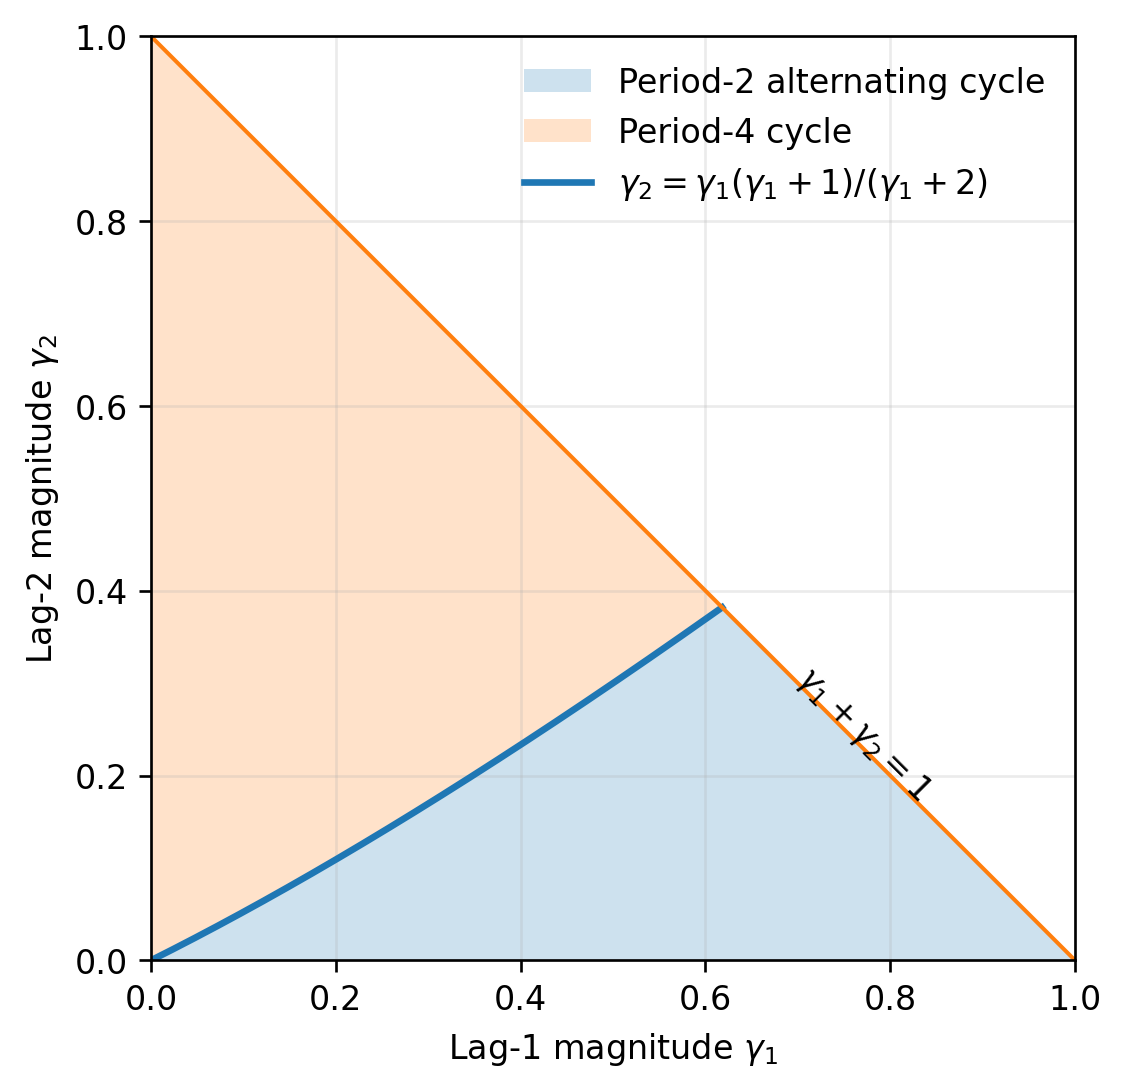
\includegraphics[width=0.72\textwidth]{figures/order_two_phase_diagram.png}
\caption{Phase diagram of the purely negative gbAR(2) family in the
coefficient magnitudes $(\gamma_1,\gamma_2)$.  The boundary
\eqref{eq:order_two_boundary} separates the period-two alternating
optimum from the period-four optimum.  The diagonal edge of the
admissible region is $\gamma_1+\gamma_2=1$, corresponding to
vanishing noise weight.}
\label{fig:order_two_phase_diagram}
\end{figure}

When $\gamma_1=\gamma_2=\alpha/2$ with $0<\alpha<1$, $w_1=w_2=1$ and
$w_{12}=-\log((1+\alpha)/2)$, so
\begin{equation}
\label{eq:balanced_order_two}
    h_\infty
    =\frac12\left[1-
      \log\left(\frac{1+\alpha}{2}\right)\right].
\end{equation}

The same formula covers the frustrated mixed-sign case.  If
$\alpha_1>0$ and $\alpha_2<0$, the gauge transformation maps the signs
to the purely negative pair while preserving the magnitudes.  Thus
\begin{equation}
\label{eq:mixed_order_two}
    h_\infty
    =\min\left\{
        -\log(\alpha_1+\beta/2),
        \frac{-\log(1-\beta/2)
              -\log(|\alpha_2|+\beta/2)}{2}
      \right\}.
\end{equation}
Among the four sign pairs
$(\operatorname{sgn}\alpha_1,\operatorname{sgn}\alpha_2)$, the pairs
$(+,+)$ and $(-,+)$ attain the floor by
\eqref{eq:two_lag_parity}, while $(+,-)$ and $(-,-)$ form the single
frustrated gauge class.

\paragraph{Balanced weights and endpoint lags.}
For a frustrated pair with $\gamma_a=\gamma_b$, we have
$w_a=w_b>w_{ab}$.  The optimal branch
preserves the larger lag $b$ and violates rule $a$ once per $b$ steps:
\begin{equation}
\label{eq:balanced_two_lag}
    h_\infty=w_{ab}+\frac{w_a-w_{ab}}{b}.
\end{equation}
In particular, take $p\ge2$ and place equal negative coefficients
$-\gamma$, with $0<\gamma<1/2$, at lags $1$ and $p$, so that $\beta=1-2\gamma$ and
$w_a=-\log(\gamma+\beta/2)=1$.  Writing
$w_H=w_{ab}=-\log(1-\beta/2)$, the pair is frustrated exactly for
even $p$, and
\begin{equation}
\label{eq:dual_endpoint}
    h_\infty=\frac{(p-1)w_H+1}{p}
    \qquad(p\ \text{even}),
\end{equation}
while odd $p$ is compatible and sits on the floor $w_H$.  For even
$p$, the period-$2p$ word
\[
    (10)^{p/2-1}\,11\,(01)^{p/2-1}\,00
\]
realizes the one-defect orbit of Lemma~\ref{lem:one_defect}.  It
satisfies the lag-$p$ rule always and pays one fair edge per $p$
output symbols.  Two incompatible endpoint rules therefore cost only
one fair bit per $p$ outputs, and the rate approaches the floor as
$p\to\infty$.

\paragraph{Weak coupling and circulant Max-Cut.}
Poljak and Turz\'ik studied Max-Cut on circulant graphs with edge
distances $1$ and $r$~\cite{poljak1992max}.  The balanced two-lag model meets
the same problem at weak coupling.  Read a periodic word as a
two-colouring of a cycle.  A negative lag rule is satisfied exactly
when its distance-$a$ or distance-$b$ edge crosses the cut.  There are
two such edge incidences per time step, so the fraction of cut edges is
one half of the mean number of satisfied rules.

For coprime $a<b$, the purely negative sign pair is frustrated exactly
when $a+b$ is odd.  The optimal branch then violates one rule every
$b$ steps, giving a mean of $2-1/b$ satisfied rules and asymptotic cut
density
\[
    \frac{2-1/b}{2}=1-\frac{1}{2b}.
\]
When $a+b$ is even, compatibility supplies a periodic two-colouring in
which every lag edge crosses the cut; the corresponding finite
circulant multigraph is bipartite.  The master formula extends this
cut-counting result from the first-order weak-coupling limit to the
full logarithmic cost at every coupling strength.

\paragraph{The R\'enyi curve at order two.}
Return to the negative order-two source with magnitudes
$\gamma_1,\gamma_2$.  Its full R\'enyi curve is explicit.  With
$w_0=-\log(\beta/2)$, complementation of every bit exchanges
$00\leftrightarrow11$ and $01\leftrightarrow10$ without changing edge
costs.  The Perron eigenvector, normalized to have coordinate sum one, is
unique and hence invariant
under this symmetry.  The four-state transfer matrix therefore reduces
to the two orbits
$\{00,11\}$ and $\{01,10\}$.  The resulting quotient matrix is
\[
    \widetilde M_q=
    \begin{pmatrix}
        2^{-qw_0} & 2^{-qw_{12}}\\
        2^{-qw_2} & 2^{-qw_1}
    \end{pmatrix}.
\]
For $q>0$, $q\ne1$, this gives
\begin{align}
    \lambda_q
    &=\frac12\Bigl(
        2^{-qw_0}+2^{-qw_1}
        +\sqrt{(2^{-qw_0}-2^{-qw_1})^2
               +4\,2^{-q(w_{12}+w_2)}}
      \Bigr),
      \label{eq:order_two_renyi_root}\\
    h_q&=\frac{\log\lambda_q}{1-q}.
\end{align}
As $q\to\infty$, the diagonal contribution $2^{-qw_1}$ yields the
alternating branch $w_1$, while the off-diagonal product
$2^{-q(w_{12}+w_2)}$ yields the period-four branch
$(w_{12}+w_2)/2$ in \eqref{eq:negative_order_two}.

On the crossing $2w_1=w_{12}+w_2$, all six non-loop edges
are critical.  In context order $00,01,10,11$, their adjacency
matrix is
\[
    K=\begin{pmatrix}
    0&1&0&0\\
    0&0&1&1\\
    1&1&0&0\\
    0&0&1&0
    \end{pmatrix}.
\]
Its quotient on the same complement pairs is
$\left(\begin{smallmatrix}0&1\\1&1\end{smallmatrix}\right)$,
whose positive eigenvector lifts to one of $K$.  Hence
$\rho(K)=\tau=(1+\sqrt5)/2$, and
\begin{equation}
\label{eq:golden_correction}
    h_q=h_\infty+
       \frac{h_\infty-\log\tau}{q-1}+o(q^{-1}).
\end{equation}
Away from the crossing the critical graph is a single cycle, so
$\rho(K)=1$.  On the crossing, paths can combine the competing
cycles, producing exponential growth at rate $\log\tau$.
The critical graph contains both $01\to10\to01$ and
$00\to01\to10\to00$.  It is strongly connected and has cycles
of lengths two and three, so its cyclicity is one.
Proposition~\ref{prop:block_periodicity} therefore implies that all
three corrections $H_*(n)-nh_\infty$ are eventually constant on
this boundary.  In the two open regions the critical cyclicities
are two and four; the block corrections can have smaller periods.

\subsection{Balanced negative orders three and four}

For the balanced purely negative family,
\[
    \alpha_i=-\frac{\alpha}{p},
    \qquad \beta=1-\alpha,
\]
where $0<\alpha<1$ unless an endpoint limit is stated explicitly,
the transition probability depends only on the number $m$ of previous
bits that disagree with the emitted bit.  Write
\begin{equation}
\label{eq:balanced_cost}
    P_m=\frac{1-\alpha}{2}+\frac{m\alpha}{p},
    \qquad c_m=-\log P_m.
\end{equation}

The Hamming weight $h(u)=\sum_{j=1}^p u_j$ counts the ones in
context $u$.  Emitting zero disagrees with $h(u)$ past bits;
emitting one disagrees with $p-h(u)$.  Thus
\begin{equation}
\label{eq:hamming_weight_guessability}
    g_1(u)=\frac{1-\alpha}{2}
       +\frac{\alpha}{p}\max\{h(u),p-h(u)\}.
\end{equation}

\begin{proposition}[Balanced negative orders three and four]
\label{prop:negative_three_four}
For the balanced purely negative source,
\begin{align}
    p=3:&\qquad
    h_\infty=c_2
    =-\log\left(\frac{3+\alpha}{6}\right),
    \label{eq:negative_order_three}\\
    p=4:&\qquad
    h_\infty=\frac{1+2c_3}{3},
    \qquad
    c_3=-\log\left(\frac{2+\alpha}{4}\right).
    \label{eq:negative_order_four}
\end{align}
\end{proposition}

\begin{proof}
\textit{Order three.}
The word $0011$ has two disagreements at every time and gives
the upper bound $c_2$.
To certify optimality, assign potential $c_2-c_3$ to the unanimous
contexts $000$ and $111$, and zero to the other six contexts.
The sixteen edge inequalities fall into four classes:
\begin{center}
\small
\begin{tabular}{ccc}
\toprule
Source and target & Disagreement count & Required inequality\\
\midrule
unanimous $\to$ unanimous & $0$ & $c_0\ge c_2$\\
unanimous $\to$ non-unanimous & $3$ & $c_3+(c_2-c_3)=c_2$\\
non-unanimous $\to$ non-unanimous & $1$ or $2$ & $c_1,c_2\ge c_2$\\
non-unanimous $\to$ unanimous & $1$ & $c_1+c_3-c_2\ge c_2$\\
\bottomrule
\end{tabular}
\end{center}
The last line is the only condition not immediate from the ordering of
the $c_m$.  It is
$c_1+c_3\ge2c_2$, equivalent to
\[
    P_1P_3\le P_2^2,
\]
because $c_m=-\log P_m$.  Direct expansion gives
\[
    P_2^2-P_1P_3=\frac{\alpha^2}{9}\ge0.
\]
The potential therefore proves the matching lower bound $c_2$.

\textit{Order four.}
The period-six cycle
\[
0001\to0011\to0111\to1110\to1100\to1000\to0001
\]
has disagreement counts $(3,2,3,3,2,3)$.  Since $c_2=1$, its mean is
$(1+2c_3)/3$.

A compact certificate separates the combinatorics from the parameter
$\alpha$.  Convexity of
$m\mapsto c_m$ means that the slopes of its piecewise linear
interpolation are nondecreasing.  The line through the adjacent points
$(2,c_2)=(2,1)$ and $(3,c_3)$ is therefore a supporting line, so
\begin{equation}
\label{eq:p4_supporting_line}
    c_m\ge1+(m-2)(c_3-1),
    \qquad m=0,\ldots,4.
\end{equation}
For an edge $u\xrightarrow{x}v$, let $m(u,x)$ be the number of bits of
$u$ different from $x$.  In lexicographic context order
$0000,0001,\ldots,1111$, take
\[
\Phi=(0,-4,-1,-5,\;0,-2,-3,-3,\;-3,-3,-2,0,\;-5,-1,-4,2).
\]
Every edge $u\xrightarrow{x}v$ satisfies
\begin{equation}
\label{eq:p4_integer_certificate}
    3m(u,x)+\Phi(v)-\Phi(u)\le8.
\end{equation}
The ordered pairs of left sides, for $x=0$ and $x=1$, in lexicographic
context order are
\[
\begin{split}
 &(0,8),(6,8),(4,8),(8,8),(0,6),(6,8),(4,8),(8,8),\\
 &(6,8),(8,4),(8,6),(6,0),(8,8),(8,4),(8,6),(6,0).
\end{split}
\]
The vector $\Phi$ is a potential for the disagreement count.  Summing
\eqref{eq:p4_integer_certificate} around a cycle of length $L$ cancels
its potential differences and gives $3\sum m\le8L$.  Thus the mean
disagreement count $\overline m$ satisfies $\overline m\le8/3$.  Thus no periodic word can disagree with more
than $8/3$ of its previous four bits on average.

Now average \eqref{eq:p4_supporting_line} around the same cycle.
Since $c_3<1$, the slope $c_3-1$ is negative, and the upper bound on
$\overline m$ becomes the lower cost bound
\[
    \overline c
    \ge1+(\overline m-2)(c_3-1)
    \ge\frac{1+2c_3}{3}.
\]
The period-six cycle attains equality.
\end{proof}

The order-four certificate bounds the mean disagreement count,
and the minimizing word attains the convex cost bound by using only
the adjacent levels two and three.  At higher orders, candidate
words use a wider range of disagreement counts.

\subsection{The balanced negative family at general order}
\label{subsec:two_run}

For $p\ge2$, consider the periodic word $0^R1^R$, with integer run
length $R$ satisfying
$\lfloor p/2\rfloor+1\le R\le p$.  During either run, the disagreement
count has $p-R+1$ occurrences of $R$ and one occurrence of each
integer from $p-R+1$ to $R-1$.  Its mean cost is therefore
\begin{equation}
\label{eq:two_run_cost}
    H_{p,R}(\alpha)
    =\frac{
       \displaystyle\sum_{m=p-R+1}^{R-1}c_m(\alpha)
       +(p-R+1)c_R(\alpha)}{R},
\end{equation}
where
\[
    c_m(\alpha)
    =-\log\left(\frac{1-\alpha}{2}+\frac{m\alpha}{p}\right).
\]
For example, when $p=5$ and $R=4$, the counts during either half of
$00001111$ are $(4,4,3,2)$.  Formula~\eqref{eq:two_run_cost} then gives
$(c_2+c_3+2c_4)/4$.

The mean number of disagreements of this word is
\begin{equation}
\label{eq:two_run_mean}
    \overline m_{p,R}
    =2p+1-R-\frac{p(p+1)}{2R}.
\end{equation}
Since
\[
    \overline m_{p,R+1}-\overline m_{p,R}
    =-1+\frac{p(p+1)}{2R(R+1)},
\]
a first-order weak-coupling optimizer within the two-run class is
\begin{equation}
\label{eq:two_run_weak_optimizer}
    R_{\mathrm{wc}}(p)
    =\left\lceil
       \frac{\sqrt{1+2p(p+1)}-1}{2}
      \right\rceil,
\end{equation}
with a tie at the next integer only when
$R_{\mathrm{wc}}(R_{\mathrm{wc}}+1)=p(p+1)/2$.  In particular,
$R_{\mathrm{wc}}(p)/p\to1/\sqrt2$.

\begin{conjecture}[Two-run envelope]
\label{conj:two_run}
For every $p\ge2$ and $0<\alpha<1$, the balanced purely negative
gbAR($p$) source satisfies
\begin{equation}
\label{eq:two_run_conjecture}
    h_\infty(\alpha)
    =\min_{\lfloor p/2\rfloor+1\le R\le p}
      H_{p,R}(\alpha).
\end{equation}
\end{conjecture}

The right side is an upper bound for every $p$, and equality holds
through order four by the formulas above.  For each
$\alpha\in\{0.2,0.5,0.8\}$, Karp computations agree through $p=13$,
and floating-point reduced-cost potentials support equality through
$p=24$.  These are checks at the stated parameter values.
Figure~\ref{fig:two_run_envelope} shows the candidate branches at
$p=12$.  The minimizing run length changes from $R=9$ to $R=8$
near $\alpha=0.484$.

\begin{figure}[tbp]
\centering
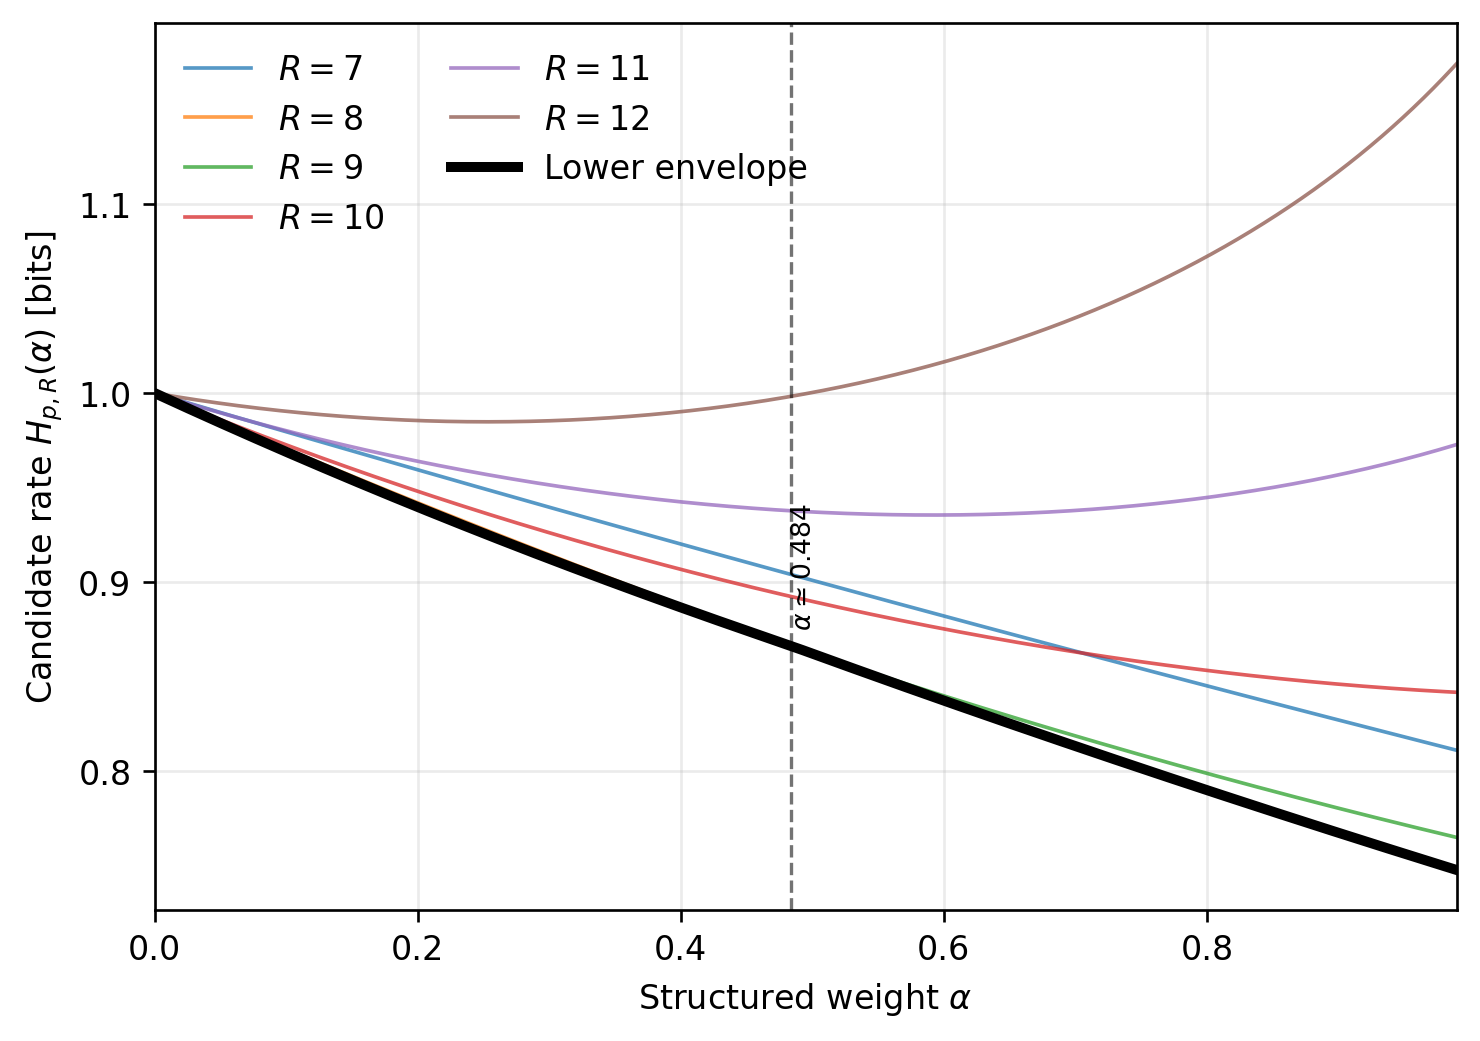
\includegraphics[width=0.82\textwidth]{figures/two_run_envelope_p12.png}
\caption{Two-run candidate rates $H_{12,R}(\alpha)$ for
$R=7,\ldots,12$.  The thick curve is their lower envelope.  The branch
crossing shows why no single run ratio describes the whole parameter
range.}
\label{fig:two_run_envelope}
\end{figure}

\paragraph{Why mean defects alone do not suffice.}
For a periodic word $y$, let $D_y$ be the number of defects at a
uniformly chosen phase.  At $p=5$, the sorted defects of $0000111$
and $00001111$ are, respectively,
\[
    (1,1,2,2,2,2,3),\qquad (1,1,1,1,2,2,3,3).
\]
The equal-run word has smaller mean defect, but
\[
    \mathbb E(D_{00001111}-2)_+=\frac14
    >\frac17=\mathbb E(D_{0000111}-2)_+.
\]
Thus the two defect distributions are incomparable in
increasing-convex order, which compares expectations of all increasing
convex functions~\cite{shaked2007stochastic}.  Nevertheless, the
equal-run word has smaller logarithmic cost.  The equal- and unequal-run
costs are, respectively,
\[
    \frac{c_2+c_3+2c_4}{4},\qquad
    \frac{c_2+4c_3+2c_4}{7}.
\]
Their comparison reduces to $c_2+2c_4\le3c_3$.  To verify it, put
$z=P_3=(5+\alpha)/10$ and $t=\alpha/5$, so
$P_2=z-t$ and $P_4=z+t$.  Then
\[
    P_2P_4^2-P_3^3=t(z^2-zt-t^2)>0,
\]
because $0<t/z<1/3$ for $0<\alpha<1$.
A proof of the conjecture must therefore use more than universal
increasing-convex domination of the defect profiles.

\begin{proposition}[Continuum two-run envelope]
\label{prop:continuum_two_run}
Fix $0<\alpha<1$.  For $x\in[0,1]$, define
\[
    f_\alpha(x)=-\log\left(\frac{1-\alpha}{2}+\alpha x\right).
\]
For a limiting run ratio $r\in[1/2,1]$, set
\begin{equation}
\label{eq:continuum_envelope}
    \mathcal H_\alpha(r)=\frac1r\left[
        \int_{1-r}^{r}f_\alpha(x)\,dx+(1-r)f_\alpha(r)
    \right].
\end{equation}
This function has a unique minimizer $r_*(\alpha)\in(1/2,1)$,
which is locally real analytic in $\alpha$.  As $p\to\infty$,
\begin{equation}
\label{eq:continuum_limit}
    \min_{\lfloor p/2\rfloor+1\le R\le p}H_{p,R}(\alpha)
    =\mathcal H_\alpha(r_*(\alpha))+O_\alpha(p^{-1}),
\end{equation}
where the error constant may depend on $\alpha$.  Every choice of
minimizing integer run lengths $R_p$ satisfies
$R_p/p\to r_*(\alpha)$.

An explicit expression is obtained by defining
\[
    z_\alpha(x)=\frac{1-\alpha}{2}+\alpha x,\qquad
    F_\alpha(x)=\frac{z_\alpha(x)[1-\ln z_\alpha(x)]}{\alpha\ln2}.
\]
Then
\begin{equation}
\label{eq:continuum_closed_form}
    \mathcal H_\alpha(r)=
    \frac{F_\alpha(r)-F_\alpha(1-r)+(1-r)f_\alpha(r)}r.
\end{equation}
The entropy extends continuously to $\alpha=0$, where it is one.
As $\alpha\downarrow0$,
\begin{equation}
\label{eq:continuum_weak}
    \min_r\mathcal H_\alpha(r)
    =1-\frac{3-2\sqrt2}{\ln2}\alpha+O(\alpha^2),
    \qquad r_*(\alpha)\longrightarrow\frac1{\sqrt2}.
\end{equation}
At this limiting ratio, the normalized mean satisfaction tends to
$2-\sqrt2$ and the complementary defect fraction to $\sqrt2-1$.
\end{proposition}

\begin{proof}
Put $r=R/p$ in \eqref{eq:two_run_cost} and divide its numerator
and denominator by $p$.  The sum becomes
\[
    \frac1p\sum_{m=p-R+1}^{R-1}f_\alpha(m/p),
\]
a Riemann sum for $\int_{1-r}^{r}f_\alpha(x)\,dx$.
The repeated endpoint contributes
$(1-r+1/p)f_\alpha(r)$.
Since $f_\alpha$ and its derivative are bounded on $[0,1]$,
\[
    H_{p,R}(\alpha)=\mathcal H_\alpha(R/p)+O_\alpha(p^{-1})
\]
uniformly over all allowed $R$.  The grid of ratios has spacing
$1/p$, and $\mathcal H_\alpha$ has bounded derivative on $[1/2,1]$.
Thus its discrete and continuous minimum values differ by
$O_\alpha(p^{-1})$.  Also $F_\alpha'=f_\alpha$, proving
\eqref{eq:continuum_closed_form}.

To locate the minimum, let
\[
    A_\alpha(r)=\int_{1-r}^{r}f_\alpha(x)\,dx+(1-r)f_\alpha(r).
\]
Differentiation gives
\begin{align*}
    A_\alpha'(r)&=f_\alpha(1-r)+(1-r)f_\alpha'(r),\\
    A_\alpha''(r)&=-f_\alpha'(1-r)-f_\alpha'(r)
                      +(1-r)f_\alpha''(r)>0,
\end{align*}
since $f_\alpha'<0$ and $f_\alpha''>0$.
Define $N_\alpha(r)=rA_\alpha'(r)-A_\alpha(r)$.  Then
$\mathcal H_\alpha'(r)=N_\alpha(r)/r^2$ and
$N_\alpha'(r)=rA_\alpha''(r)>0$, whereas
\[
    N_\alpha(1/2)=\tfrac14 f_\alpha'(1/2)<0,\qquad
    N_\alpha(1)=f_\alpha(0)-\int_0^1 f_\alpha(x)\,dx>0.
\]
There is exactly one zero, and it is the unique minimizer.
The analytic implicit function theorem applies because this zero is
simple.  Uniform convergence of the discrete costs then forces every
subsequential limit of $R_p/p$ to equal $r_*(\alpha)$, proving
convergence of the minimizers.

Finally, the expansion
$f_\alpha(x)=1-(2x-1)\alpha/\ln2+O(\alpha^2)$ is uniform in $x$.
Substitution gives, uniformly in $r$,
\[
    \mathcal H_\alpha(r)=
    1-\left(3-2r-\frac1r\right)\frac{\alpha}{\ln2}+O(\alpha^2).
\]
The bracket has its unique maximum $3-2\sqrt2$ at $r=1/\sqrt2$.
This proves \eqref{eq:continuum_weak}, including convergence of the
minimizers by compactness.  Substituting this ratio into
$\overline m_{p,R}/p\to2-r-1/(2r)$ gives the stated satisfaction
and defect fractions.
\end{proof}

These continuum statements concern the two-run candidate and do not
assume Conjecture~\ref{conj:two_run}.

\subsection{Summary and computational audit}

Table~\ref{tab:family_summary} collects the uniform-noise formulas.

\begin{table}[htbp]
\centering
\caption{Closed and conjectural gbAR min-entropy rates.  Here
$w_H=-\log(1-\beta/2)$, the two-lag costs $w_a,w_b$ are defined in
Section~\ref{subsec:two_lag}, and $c_m$ is defined in
\eqref{eq:balanced_cost}.}
\label{tab:family_summary}
\footnotesize
\setlength{\tabcolsep}{4pt}
\renewcommand{\arraystretch}{1.12}
\begin{tabular}{p{0.27\textwidth}p{0.29\textwidth}p{0.35\textwidth}}
\toprule
\textbf{Family} & \textbf{Conditions} & $\boldsymbol{h_\infty}$\\
\midrule
Positive gbAR & $\alpha_i\ge0$ & $w_H$ for uniform noise\\
Single active lag & one nonzero coefficient & $w_H$\\
Alternating signs & even $p$ & $w_H$\\
\midrule
Two active lags, compatible & $as_b+bs_a\equiv0\pmod2$ after compression &
$w_H$\\
Two active lags, frustrated & $as_b+bs_a\equiv1\pmod2$ for coprime $a<b$ &
$\min\{((a-1)w_H+w_a)/a,\ ((b-1)w_H+w_b)/b\}$\\
\quad order two & $(a,b)=(1,2)$ &
$\min\{w_1,(w_{12}+w_2)/2\}$\\
\quad endpoint lags & even $p$, equal weights at lags $1,p$ &
$((p-1)w_H+1)/p$\\
\midrule
Balanced negative gbAR(3) & $\alpha_i=-\alpha/3$ &
$-\log((3+\alpha)/6)$\\
Balanced negative gbAR(4) & $\alpha_i=-\alpha/4$ &
$(1+2c_3)/3$\\
Balanced negative gbAR($p\ge5$) & $\alpha_i=-\alpha/p$ &
$\min_R H_{p,R}$, conjectural\\
Odd alternating signs & odd $p$ &
same as balanced negative order $p$\\
\bottomrule
\end{tabular}
\end{table}

The accompanying code checks the
floor criterion through order five, the closed families, the order-four
integer certificate, and the two-run envelope.  Running
\texttt{python3 repo/verify.py} with \texttt{--karp-max-order 13}
and \texttt{--karp-workdir /tmp} reproduces the full-graph comparisons at
$\alpha\in\{0.2,0.5,0.8\}$.
The separate script \texttt{experiments/verify\_two\_lag\_master.py}
checks 384 frustrated lag-sign-weight configurations against Karp's
algorithm and exhaustively checks 393,192 periodic words of lengths
one through fourteen across twelve frustrated lag-sign choices.
The covering inequality is attained in every choice.

The C program \texttt{repo/two\_run\_certificate.c}, run with
\texttt{--max-order 24}, constructs reduced-cost potentials and checks
every edge for orders two through twenty-four at the same three
couplings.  It uses double precision and accepts slack down to
$-10^{-9}$.  These checks are numerical evidence, not rigorous
finite-block certificates; the latter require verified error bounds
as in Corollary~\ref{cor:finite_block_certificate}.
The script \texttt{repo/generate\_figures.py} reproduces
Figures~\ref{fig:order_two_phase_diagram} and
\ref{fig:two_run_envelope}.

\section{Conclusion}
\label{sec:conclusion}

For binary sources with finite memory, the minimum mean cycle gives
an exact entropy rate, and an edge potential certifies finite-block
lower bounds.  The critical graph also determines the leading
large-order R\'enyi correction and the eventual periodicity of block
costs.  At the order-two branch crossing, its spectral radius is the
golden ratio and its cyclicity is one.

For parity-rule mixtures, a polynomial gcd decides whether the noise
floor is attained.  Every incompatible system has a two-rule witness,
and counting its translated defects gives weighted entropy gaps and
finite-block bounds.  These bounds are attained for every two-lag
gbAR source.  Gauge symmetry preserves all block entropies, while
profiles describe the cost of defects when more rules interact.

The balanced negative family remains open at general order.  Its
two-run candidate agrees with the computations reported here and has
a unique continuum minimizing ratio, with an explicit convergence
bound for its values.  The order-five counterexample rules out a
universal increasing-convex comparison of defect profiles.  Proving
the conjecture requires a sharper inequality for the logarithmic cost
or an all-order potential.  More generally, the gap between pairwise
covering bounds and realizable defect profiles is the remaining
obstacle for mixtures of three or more rules.

\section*{AI assistance}
The research vision and original ideas are the author's. The author used OpenAI's GPT models, including Astra, and Anthropic's Claude Opus models for writing, theorem proving, and literature review. GPT models were used most often, and Astra was the most useful overall. This work is in progress. Not all claims have been verified by a human.

\bibliographystyle{unsrt}
\bibliography{references}
\end{document}
